\documentclass{article}
\usepackage[utf8]{inputenc}

\usepackage[paperwidth=8.5in, paperheight=11in, top=1in, bottom=.5in, left=.5in, right=.5in]{geometry}
\usepackage{fancyhdr, graphicx,tikz,amsmath,multicol,paracol,pgfplots}
\usepackage[inline]{enumitem}
\pgfplotsset{compat=1.18}


\pagestyle{fancy}
\lhead{\large{\textbf{Module 2: Functions (FN) - Readiness Assurance Test}}}
\chead{}
\rhead{}
\lfoot{}
\cfoot{}
%\rfoot{\thepage/\pageref{LastPage} }
\setlength{\headheight}{14pt} %added in bc warning

%%% LIST ANSWER KEY HERE

% 1 B
% 2 A
% 3 D
% 4 D
% 5 B
% 6 A
% 7 D
% 8 C


\begin{document}


\begin{enumerate}


% interval notation
\item Write the inequality $x\ge -2$ in interval notation. 

        \begin{enumerate}
        \begin{multicols}{4}
          \item $(-2,\infty)$
          \item $[-2,\infty)$ %correct
          \item $(-\infty,-2]$
          \item $(-\infty,-2)$ 
        \end{multicols}
        \end{enumerate}

\item Write the expression $x\neq 3$ in interval notation. 

        \begin{enumerate}
        \begin{multicols}{4}
          \item $(-\infty,3) \cup (3,\infty)$ %correct
          \item $(3, \infty)$ 
          \item $(-\infty,3)$
          \item $(-\infty, 3] \cup [3, \infty)$ 
        \end{multicols}
        \end{enumerate}


% Evaluate a function at a given value.

\item What is the value of the expression $5(y-2x)+(2-y)^2$ when $x=-2$ and $y=3$?

  \begin{enumerate}
  \begin{multicols}{4}
  \item $20$
  \item $50$
  \item $1156$
  \item $36$ %correct
   \end{multicols}
  \end{enumerate}

% Order of operations

\item Simplify the expression $\dfrac{4-\sqrt{4^{2}-2(5)(-2)}}{2}+3$.

  \begin{enumerate}
  \begin{multicols}{4}
  \item $-1$
  \item $4$
  \item $-2$
  \item $2$ %correct
   \end{multicols}
  \end{enumerate}

% Plot points

\item Two points are graphed on the coordinate plane. Which ordered pairs represent these points?
\begin{center}
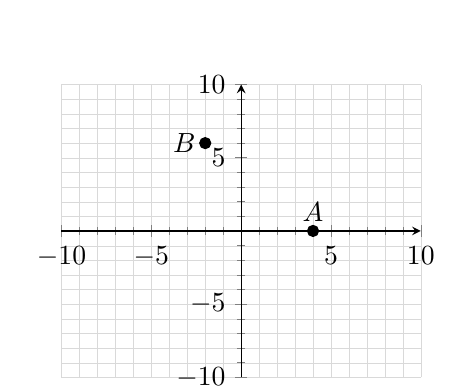
\begin{tikzpicture}
        \begin{axis}[
                height=5.3cm,
                axis lines=center,
                grid=both,
                grid style={line width=.05pt, draw=gray!30},
                minor tick num=4,
                xtick={-10,-5,...,10},
                ytick={-10,-5,...,10},
                xmin=-10, xmax=10,
                ymin=-10, ymax=10,
                ]
                \addplot[mark=*] coordinates {(4,0)} node[above ] {$A$};
                \addplot[mark=*] coordinates {(-2,6)} node[left ] {$B$};
        \end{axis}
        \end{tikzpicture}
\end{center}

  \begin{enumerate}
  \begin{multicols}{2}
  \item $A(-4,0)$ and $B(-2,-6)$  
  \item $A(4,0)$ and $B(-2,-6)$ %correct 
  \item $A(4,0)$ and $B(2,-6)$ 
  \item $A(0,-4)$ and $B(-2,-6)$
  \end{multicols}
  \end{enumerate}

%simplify an expression by combining like terms

\item Simplify the expression $(x^{2}-3x)-(x^{3}-4x^{2}+7)$.
 \begin{enumerate}
  \begin{multicols}{2}
  \item $-x^{3}+5x^{2}-3x-7$ %correct
  \item $x^{3}-3x^{2}-3x+7$
  \item $-x^{3}-3x^{2}-3x+7$
  \item $x^{2}-3x-x^{3}+4x^{2}+7$
   \end{multicols}
  \end{enumerate}  
\pagebreak
% Rewrite an equation in terms of another variable
  
\item Given the equation, $3x-4y=8$, solve for $y$ in terms of $x$.

  \begin{enumerate}
  \begin{multicols}{4}
  \item $y=8-3x$
  \item $y=8-\dfrac{3x}{4}$
  \item $y=-3x-2$
  \item $y=\dfrac{3}{4}x-2$ %correct
   \end{multicols}
  \end{enumerate}

\item Given the equation, $y=3-\sqrt{x+5}$, solve for $x$ in terms of $y$.

  \begin{enumerate}
  \begin{multicols}{4}
  \item $x=3+\sqrt{y+5}$
  \item $x=(y+3)^{2}+5$
  \item $x=(3-y)^{2}-5$ %correct
  \item $x=(y-3)^2+5$ 
   \end{multicols}
  \end{enumerate}



\end{enumerate}


\end{document}